\documentclass{amsart}

\usepackage{graphicx}
\usepackage{pdfpages}
\usepackage{pbox}
\usepackage{caption}
\usepackage[normalem]{ulem}
\usepackage{hyperref}
\usepackage{listings}
\usepackage{pdflscape}
\usepackage[pass]{geometry}

% \geometry{reset} doesn't work...get figures from log:
\geometry{textwidth=360.0pt,textheight=584.0pt}

\captionsetup[figure]{labelformat=empty}

\title{CSCI 6907 Project Final Report\\
Lights Out Management}
\author{James Lee\\
\texttt{jameslee@gwu.edu}}
\date{\today}

\begin{document}
\maketitle

\section{Project Abstract}
I am a system administrator who manages hundreds of Unix systems.  One of the essential tools to ensure I don't have to visit the datacenter every time I want to work on a system is called ``lights out management'' (LOM).  It's a little device built into high-end servers that allows me to log in over the network, power the system on and off, and access the operating system's console, when more traditional methods such as SSH fail.

I run my personal file and web server at home on a Sun Ultra 24.  It's a low-end, commodity X86 system with no built-in LOM.  I've rendered it inaccessible many times while performing upgrades or configuration changes remotely.  I could have benefitted from a LOM in my home server, so I built one.

My LOM allows me to connect to it over the network using Rlogin, power the system on and off, and access the system's serial console for every state the system is in (BIOS, bootloader, kernel boot, console login shell) all without modifying the server's hardware.

\section{Status}
The project went according to plan.  All of the milestones were completed on schedule and all of the features were implemented as proposed.

\section{Specification}
The device is built on top of the Arduino Prototyping Platform.  I chose the Arduino mostly because I already own one (an Arduino Uno) and I wanted to keep costs low.  This device is something I'll actually use, so I didn't want to borrow any components.  The Arduino was also attractive because of the availability of ``shields'' that extend its functionality by plugging new components into the board without soldering.

For network access, I chose the Freetronics Ethernet shield.  The Freetronics shield is fully compatible with the official Arduino Ethernet shield, so it can use the same Ethernet library, however it also includes extra circuitry to fix a bug in the shield's Wiznet W5100 Ethernet module that causes it to hold on to the SPI bus even when its chip select is not active.  The Freetronics shield also includes a small prototyping area that I took advantage of to keep the final device nice and compact.

The device is powered by the Arduino's USB port.  The Sun Ultra 24 has an internal USB port that always supplies power, even when the system is off.

For serial console access, I chose to implement the Maxim MAX3110E.  It's a combination of an SPI compatible UART and RS-232 transceiver.  The chip also has a 16 byte FIFO buffer and raises an interrupt when data is available.  The Arduino uses the interrupt to know when to read data from the UART.

To control the system's power, the LOM effectively sits between the pins of the physical power switch.  Then it uses an NPN transistor to act as an electronic switch.  The device detects the system's power state from the power LED.

On top of the hardware sits a simple CLI that allows a user to interact with the LOM over the Rlogin protocol.  The proposal called for using Telnet, however it turned out that Telnet was significantly more complicated than I anticipated.  Telnet is designed to work with multiple platforms and terminal types, so it defines its own terminal command set called network virtual terminal (NVT), which I would have had to convert the VT100 terminal of the serial console to.  Rlogin, by comparison, assumes like-to-like terminal types, so no terminal translation is necessary, so long as I \texttt{rlogin} from a VT100 compatible terminal.

In addition to exposing power control and serial console options, the CLI also allows the user to configure the LOM's network settings including whether or not to use DHCP.  The settings are stored persistently in the Arduino's EEPROM.

\section{Implementation \& Construction}

Implementation began with verifying the serial connection on the motherboard is functional.  I determined the header pinout by searching on the internet.  I connected wires to the RX, TX, and ground pins to a serial cable and the serial port on my laptop.  After configuring the BIOS, bootloader, etc, to output to the serial port, I was able to interact with the serial console using minicom on my laptop.

Next, while parts were on order, I set out to figure out how to tap into the power LED and switch.  I disassembled computer to pull out the front panel board.  I trace the pins and used a multimeter to infer what the board did.  Then I started prototyping different ways I could use it:

\begin{center}
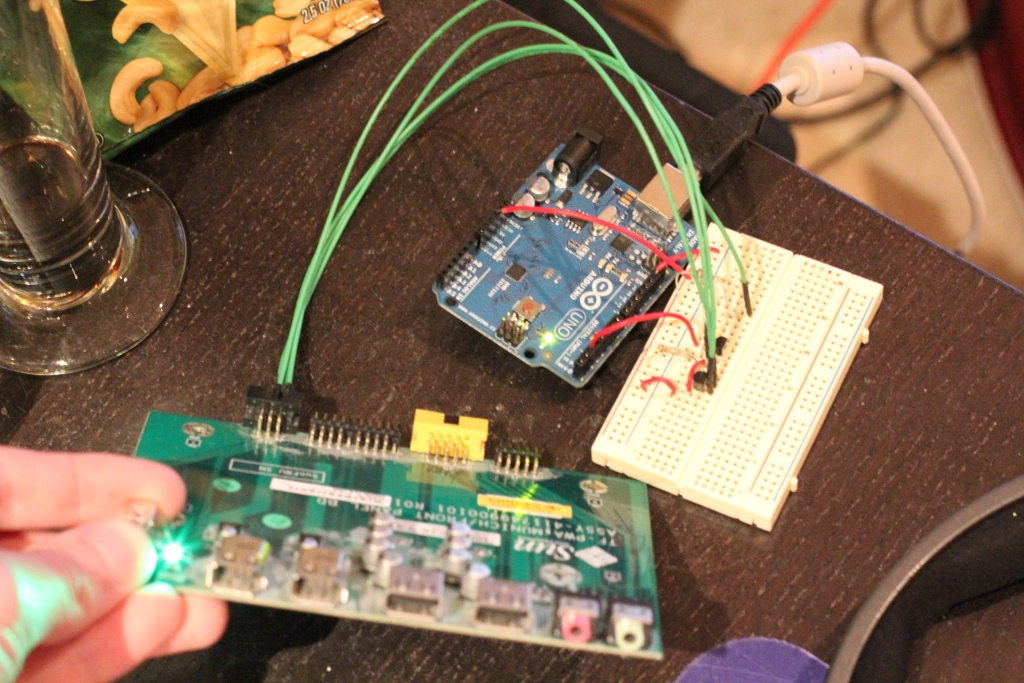
\includegraphics[width=.9\textwidth]{pled.jpg}
\end{center}

The following parts were ordered for the project:

\begin{center}
\begin{tabular}{|l|l|}
\hline
\multicolumn{1}{|c|}{\textbf{Part}} & \multicolumn{1}{|c|}{\textbf{Price}}\\
\hline
Freetronics Ethernet Shield With PoE & \$46.46\\
\hline
\pbox{5in}{Maxim MAX3110E\\SPI-compatible UART and RS-232 Transceiver} & \$12.89\\
\hline
$2\times$ 33pF 50V Ceramic Disc Capacitor (5\%) & \$0.18\\
\hline
\pbox{5in}{ECS 36-18-4X\\3.6864 MHz 18pF Crystal Oscillator} & \$0.53\\
\hline
\end{tabular}
\end{center}

I also ordered a couple of optocouplers to use to connect the Arduino to the system's power control headers, but after testing with the multimeter, I determined that it would be safe to connect the Arduino directly.

\begin{center}
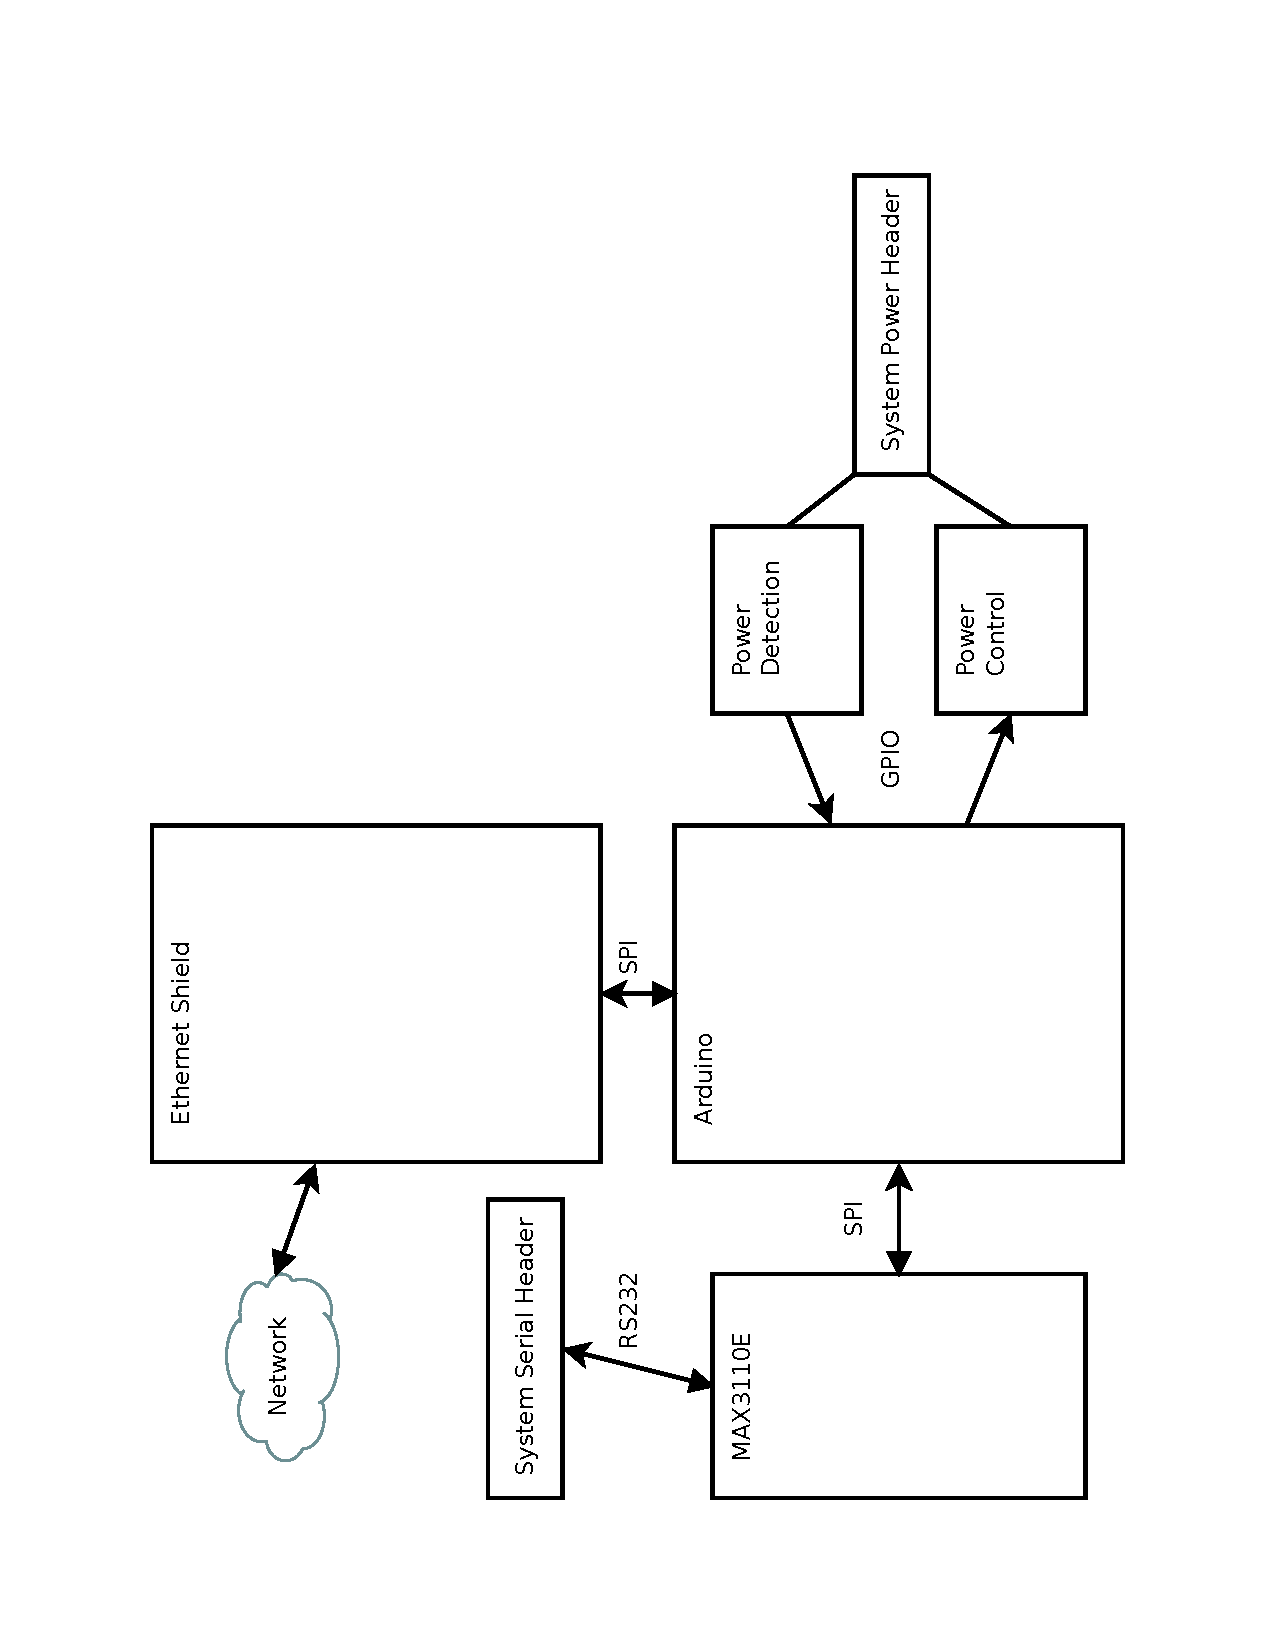
\includegraphics[height=\textwidth,angle=270]{hw-block.pdf}
\end{center}

Next I drafted a schematic based on the MAX3110 datasheet and what I learned about the power control board.

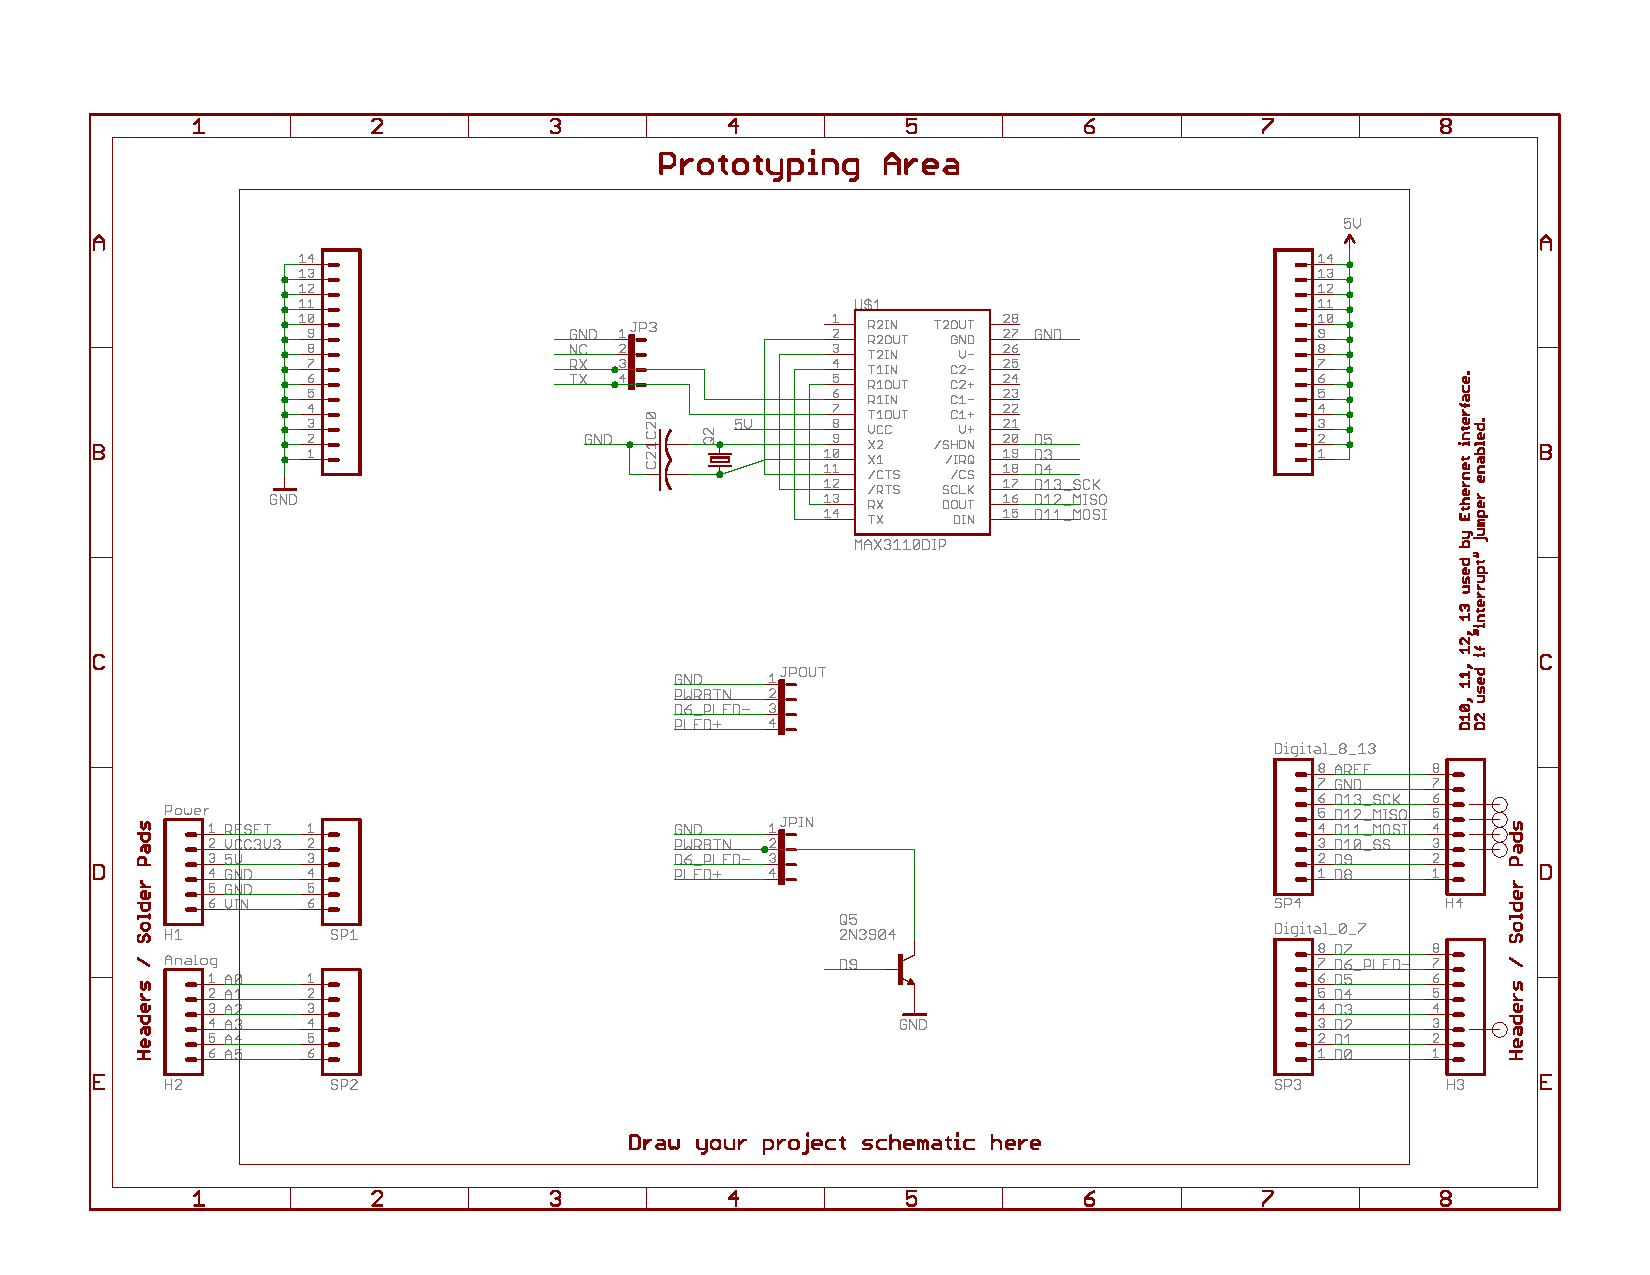
\includepdf[landscape]{schematic.pdf}

I constructed the project on a breadboard to start:

\begin{center}
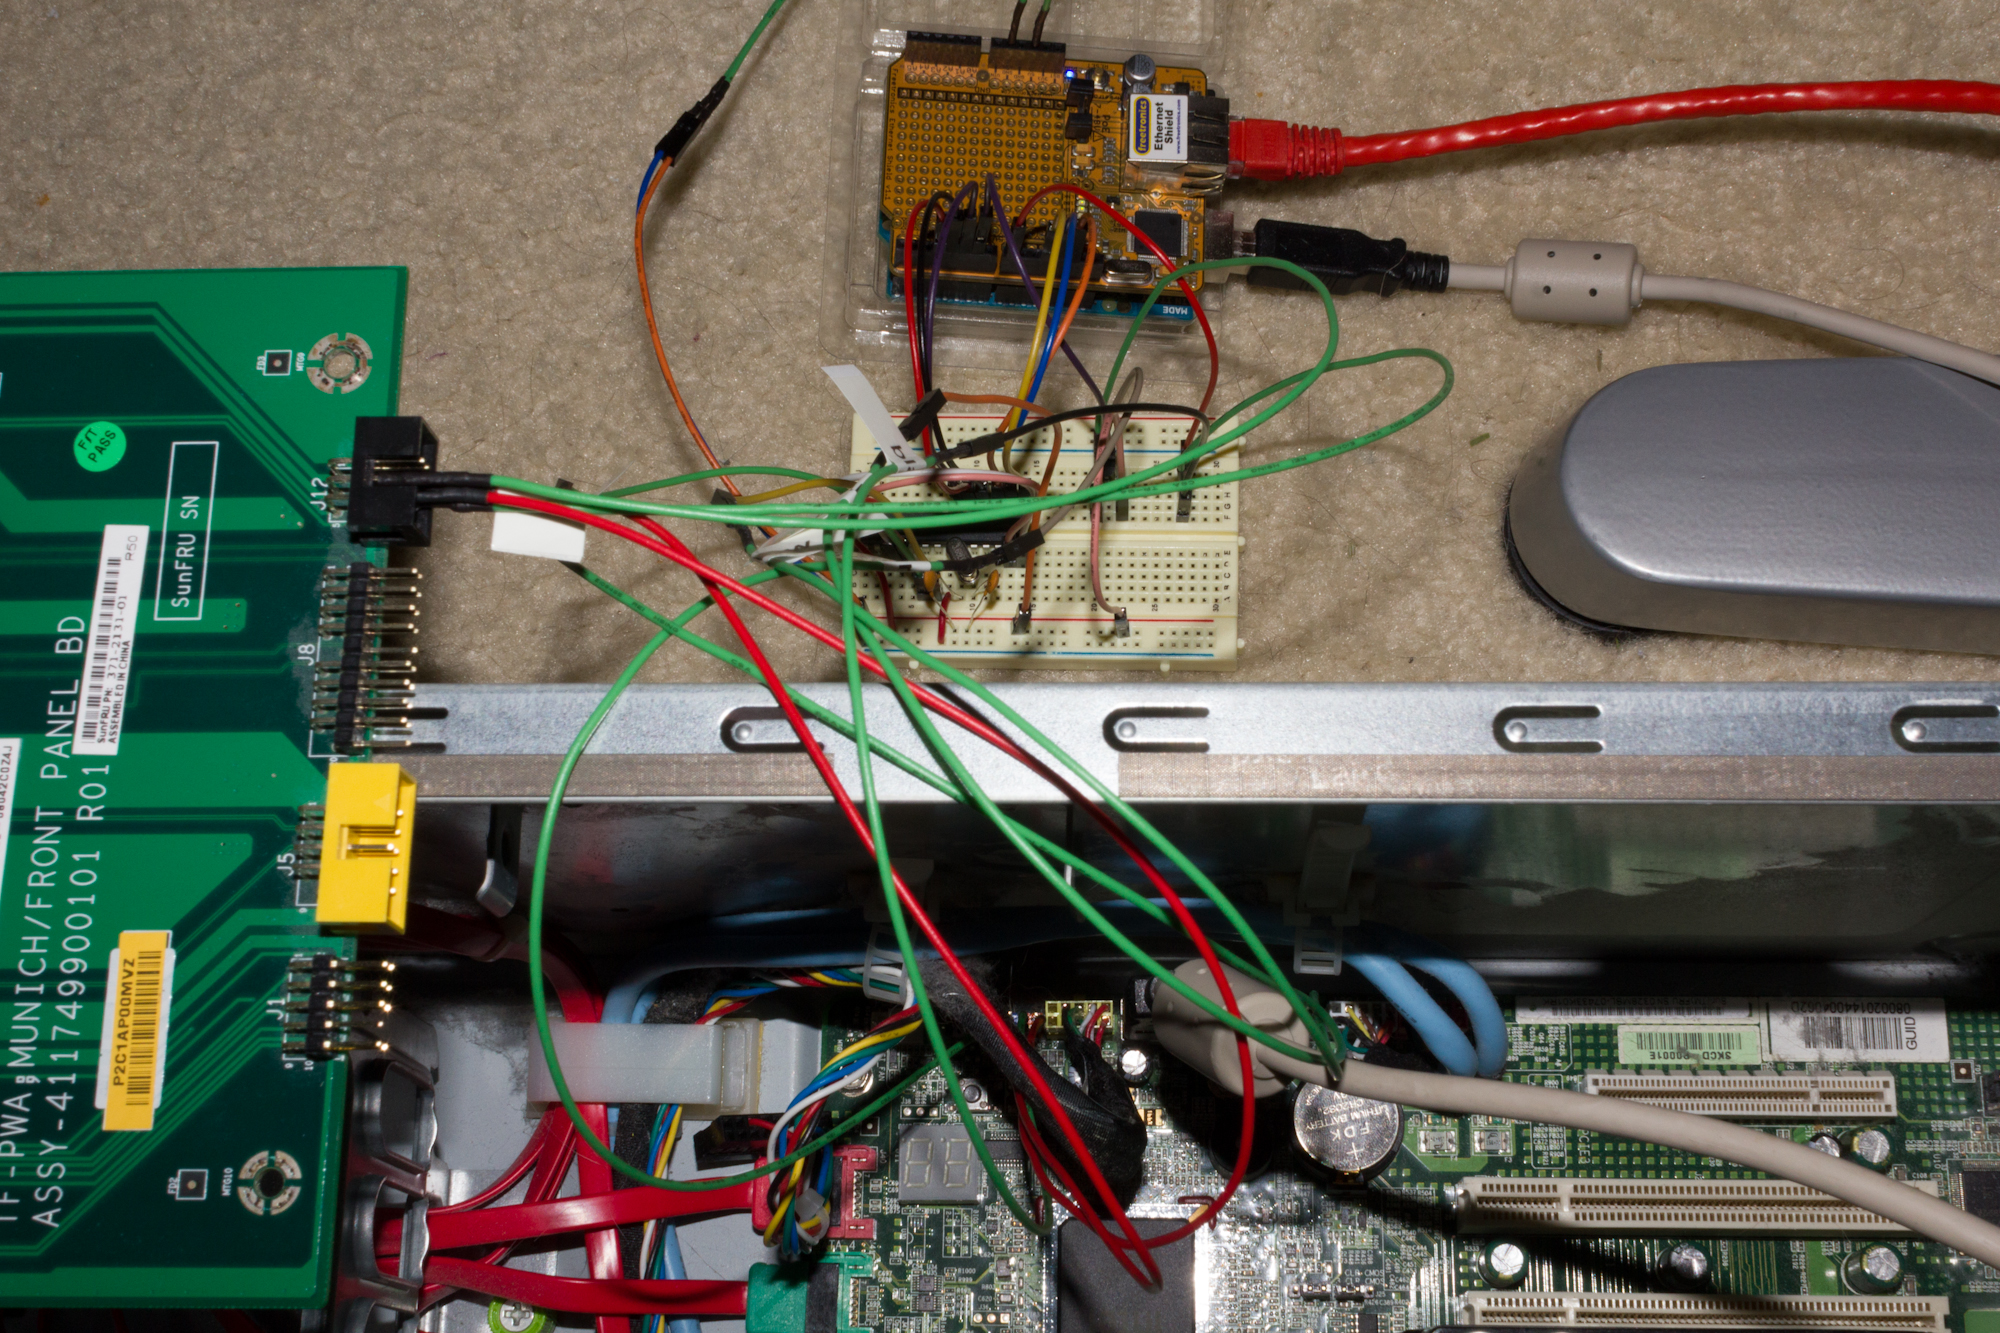
\includegraphics[width=.9\textwidth]{lom-02.jpg}
\end{center}

Then I began writing the code, starting with the implementing the MAX3110 chip, then implementing the \sout{Telnet} Rlogin server and CLI (adapted from Lab 3), and finally the power control, bringing it all together at the end.  You can see how the code evolved at \url{https://github.com/MrStaticVoid/school/commits/master/CSCI6907/project/sketch}.

One of the goals that I achieved was to implement the code in a way that is consistent with the rest of the Arduino library.  For example, for the MAX3110 driver I wrote, I extended the \href{http://arduino.cc/en/Reference/Stream}{Stream} class similar to the software serial library such that I only had to implement a few virtual functions:

\begin{quote}
\lstset{language=C++,basicstyle=\footnotesize,breaklines=true}
\begin{lstlisting}
class Max3110 : public Stream {
    public:
        Max3110(uint8_t ssPin, uint8_t shutdownPin, uint8_t interruptPin, uint8_t interruptNum);
        void begin(unsigned long baud);
        void end();
        virtual size_t write(uint8_t b);
        virtual int available();
        virtual int read();
        virtual int peek();
        virtual void flush();
    ...
}

extern Max3110 ExternalSerial;
\end{lstlisting}
\end{quote}

and I got complex higher level functions such as string writing for free.  A global instance of the class is also provided so the program can use the UART from anywhere in the program like \texttt{ExternalSerial.write(...)} just as one can use the Arduino Serial class like \texttt{Serial.write(...)}.

After getting the code in order, I took the schematic and PCB sketch provided by Freetronics and figured out a way to fit everything on the prototyping area of the Ethernet shield:
\\
\begin{center}
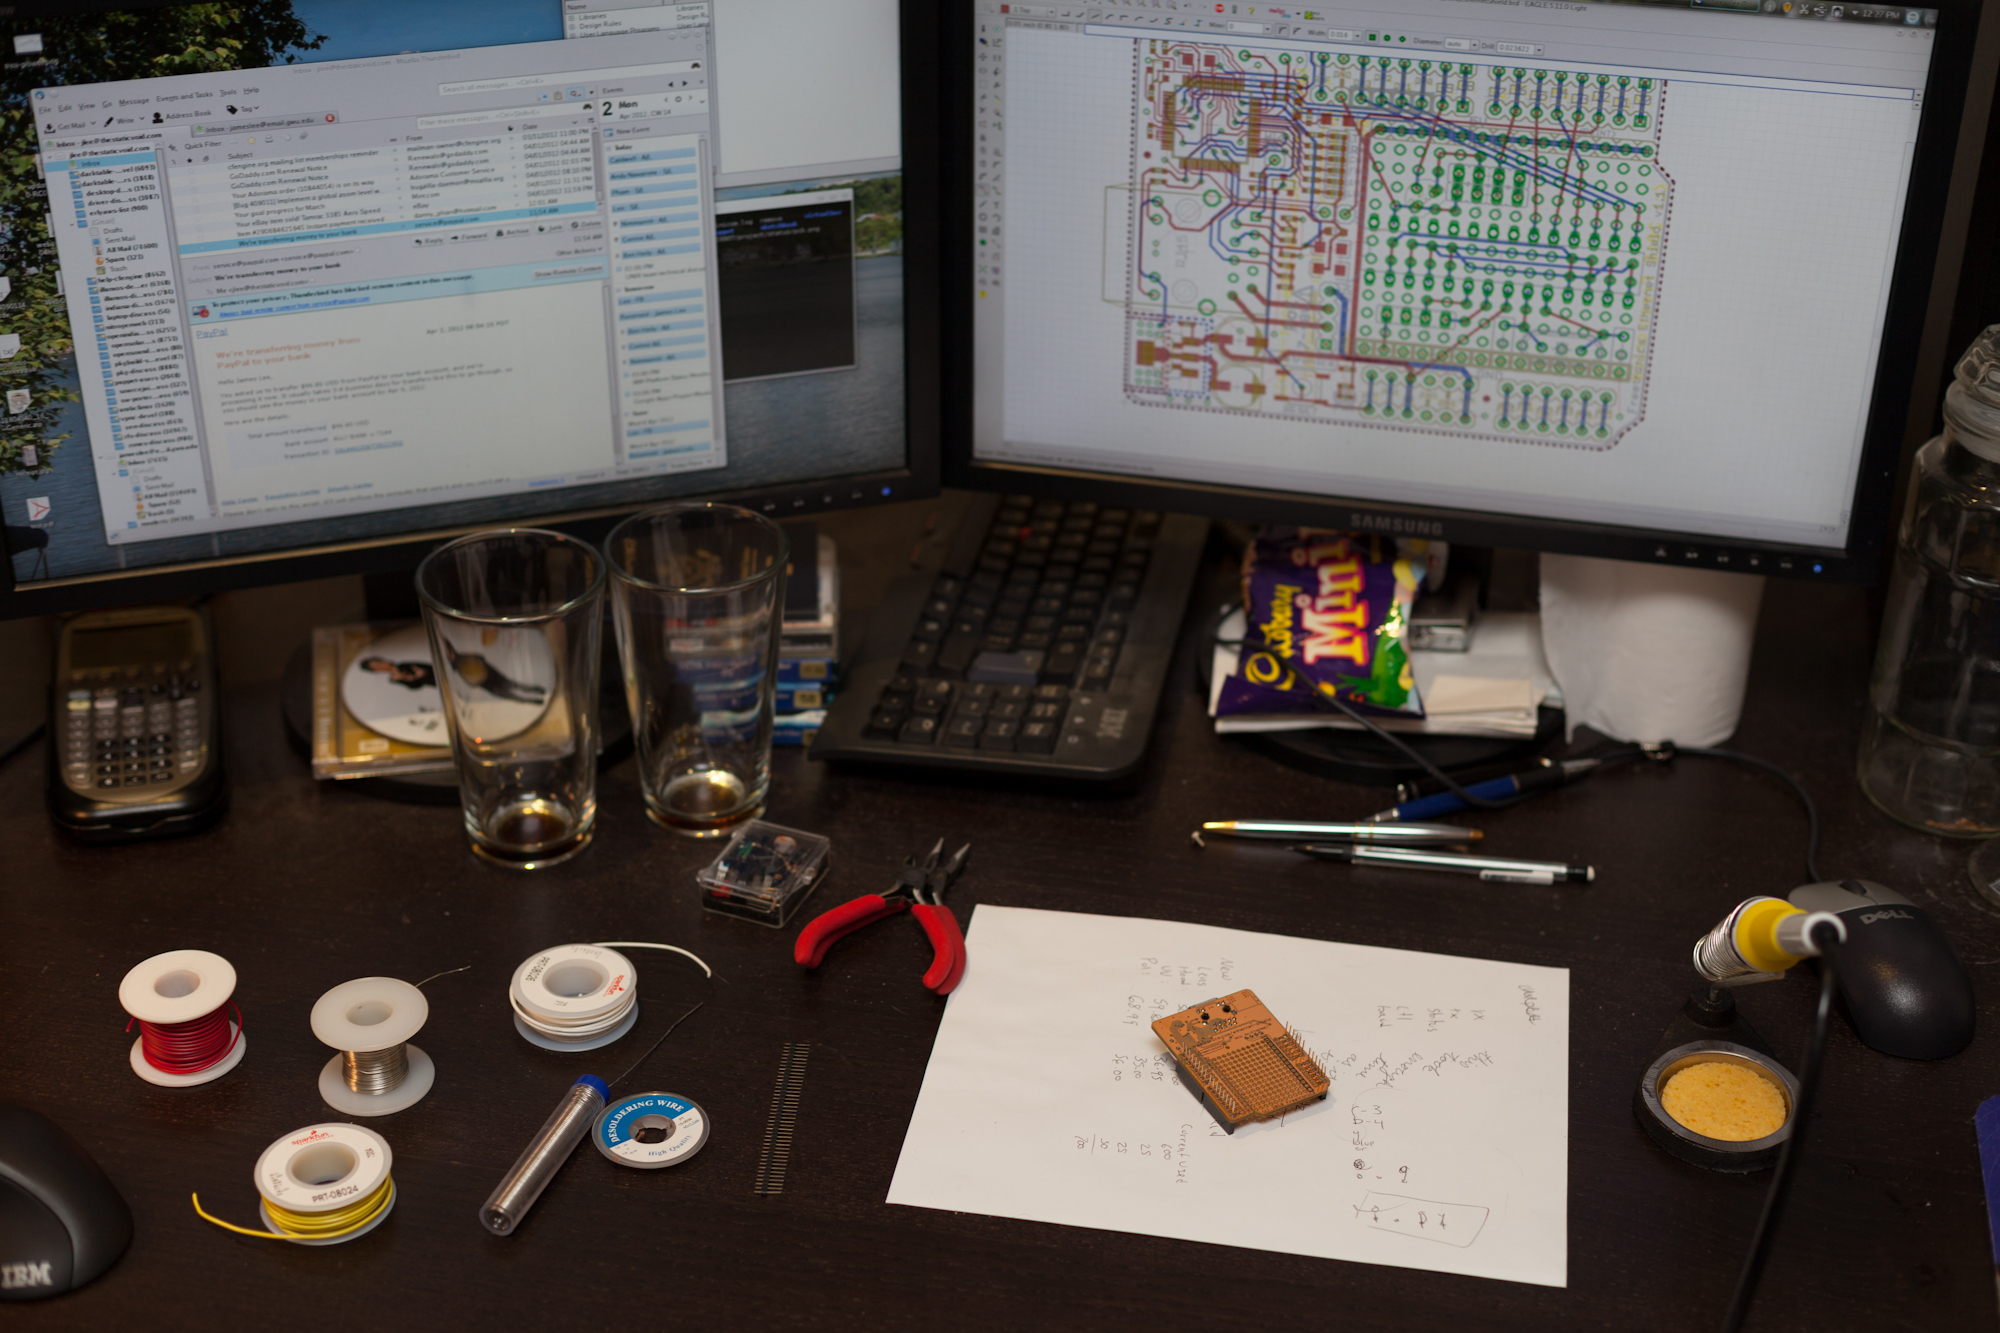
\includegraphics[width=.9\textwidth]{lom-07.jpg}
\end{center}
\ \\
\begin{center}
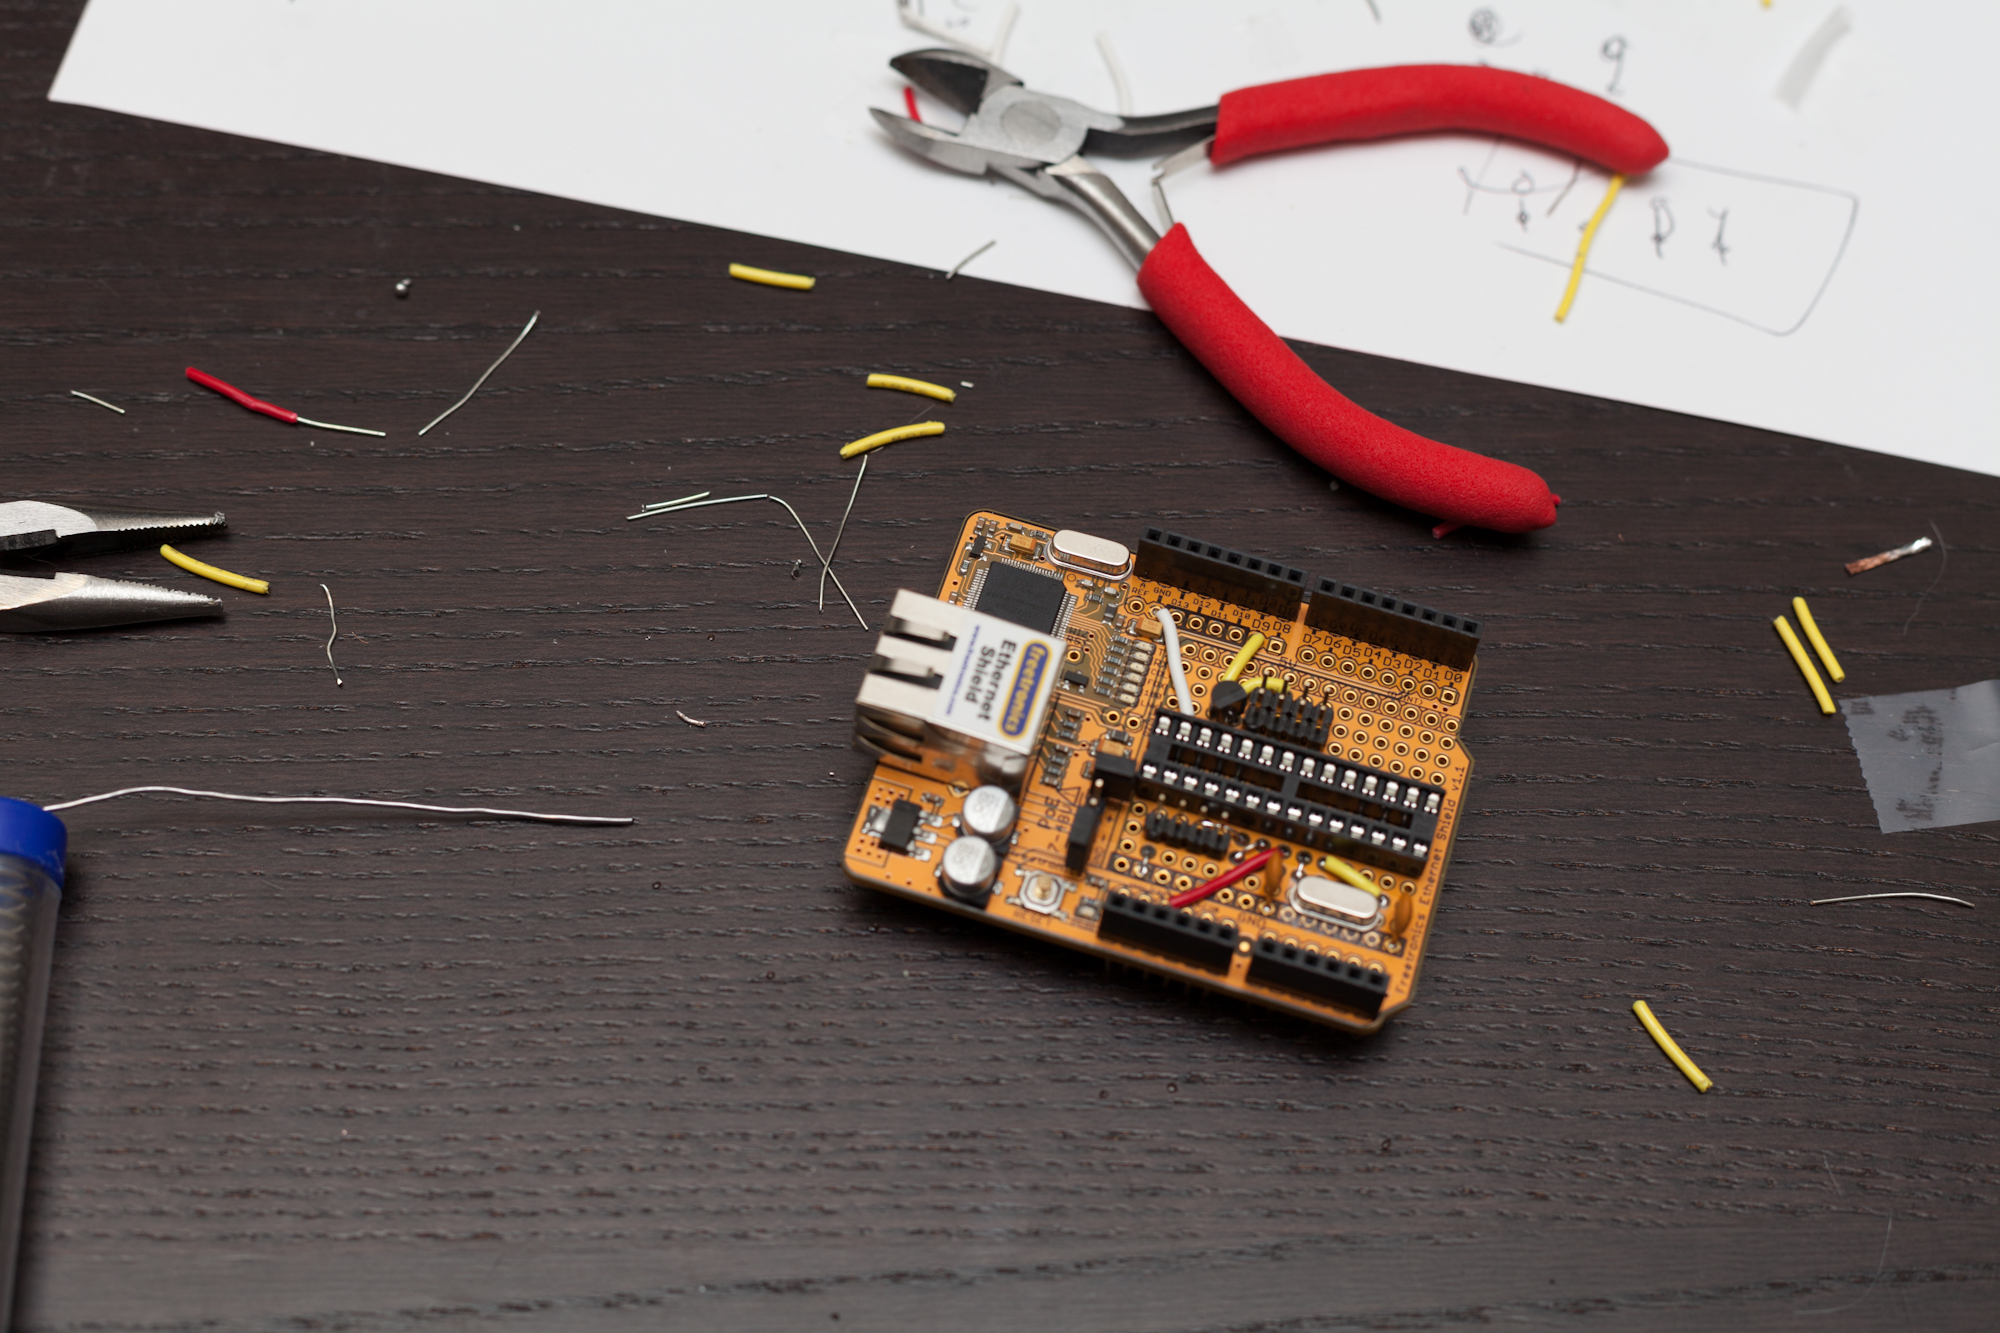
\includegraphics[width=.9\textwidth]{lom-10.jpg}
\end{center}

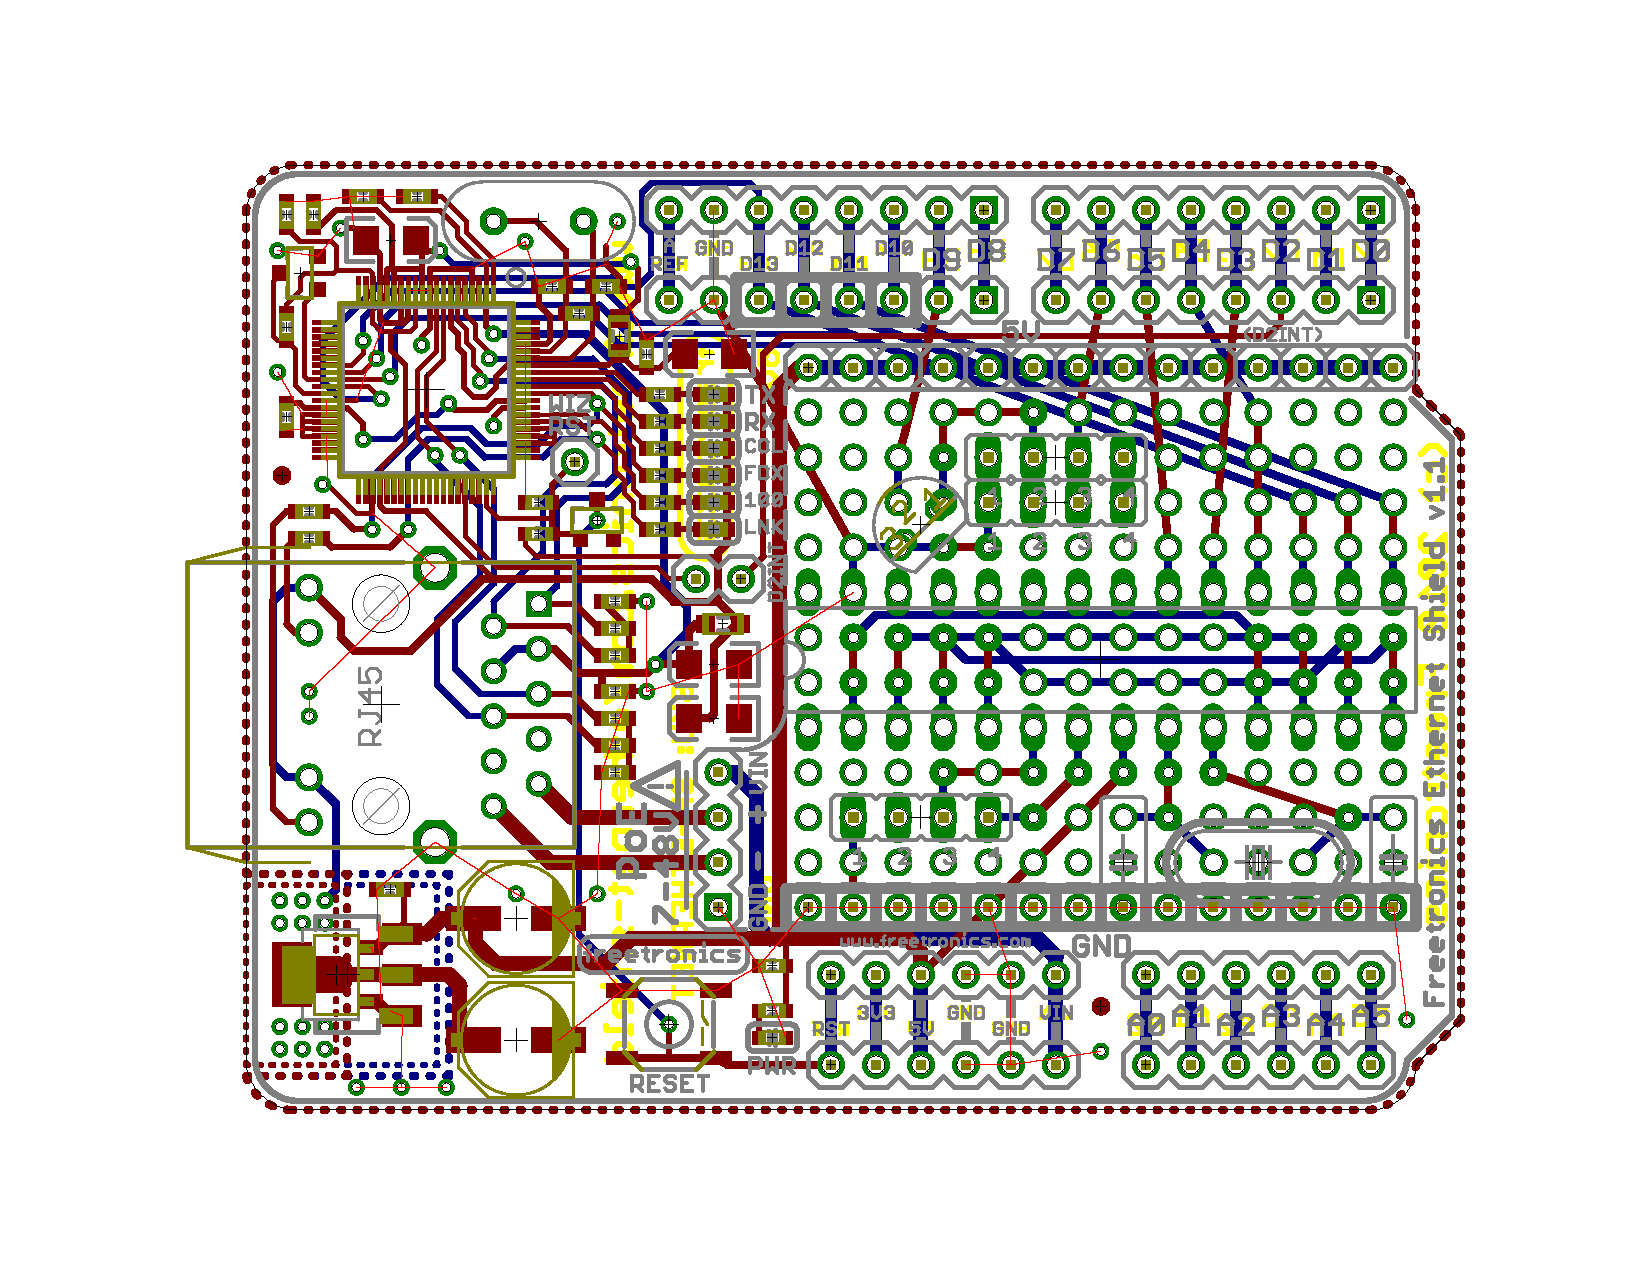
\includepdf[landscape]{pcb.pdf}

\newgeometry{margin=.5in}
\begin{landscape}
\noindent\thispagestyle{empty}
\parbox[c][\textwidth][s]{\linewidth}{%
\vfill
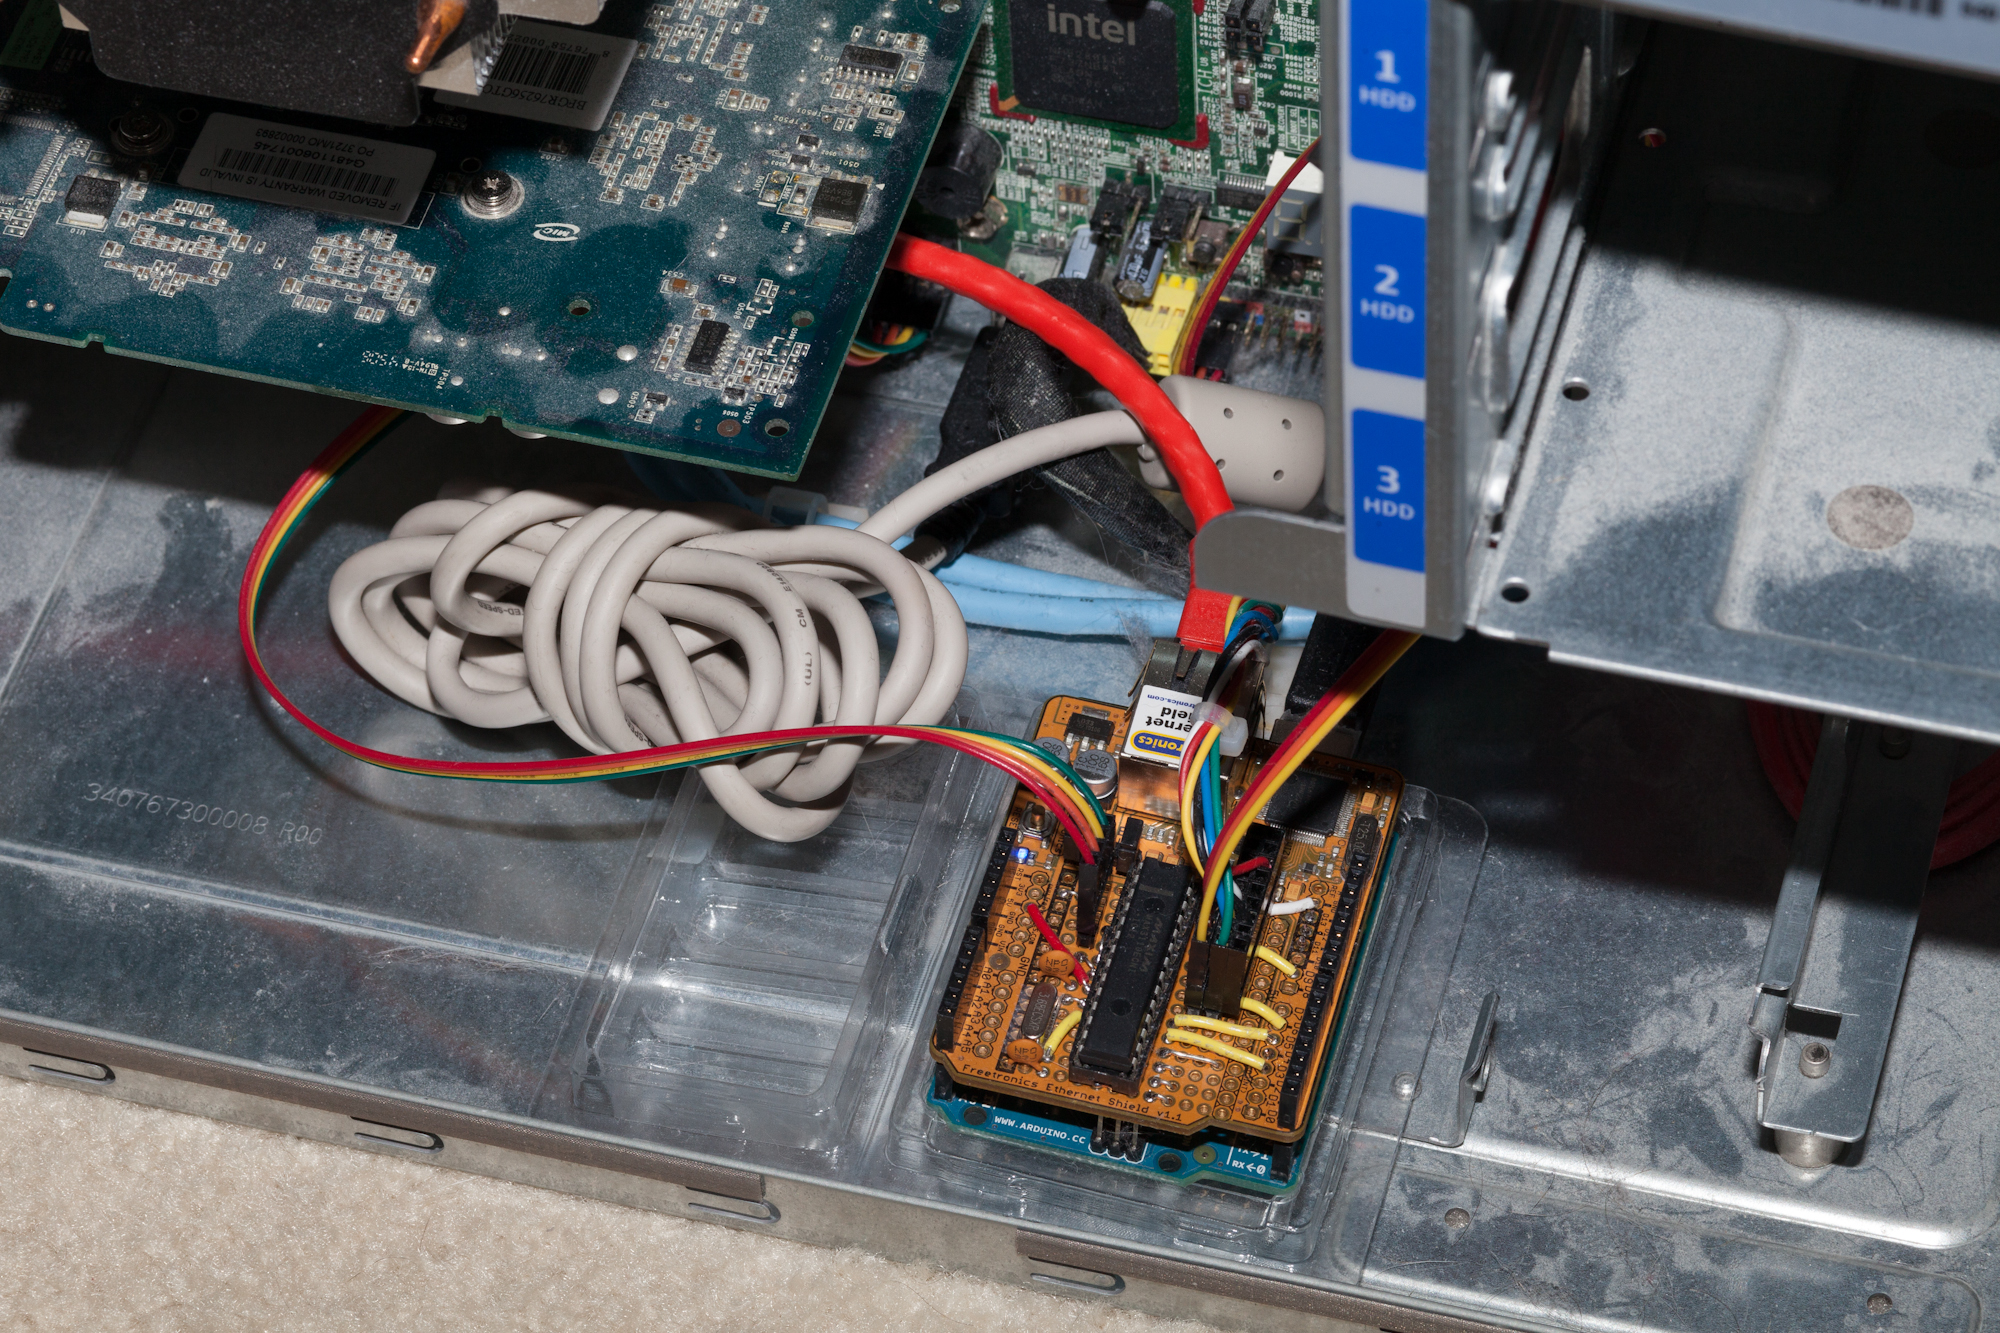
\includegraphics[width=\linewidth]{lom-14.jpg}
\vfill
}
\end{landscape}
\restoregeometry

An example LOM session:
\begin{center}
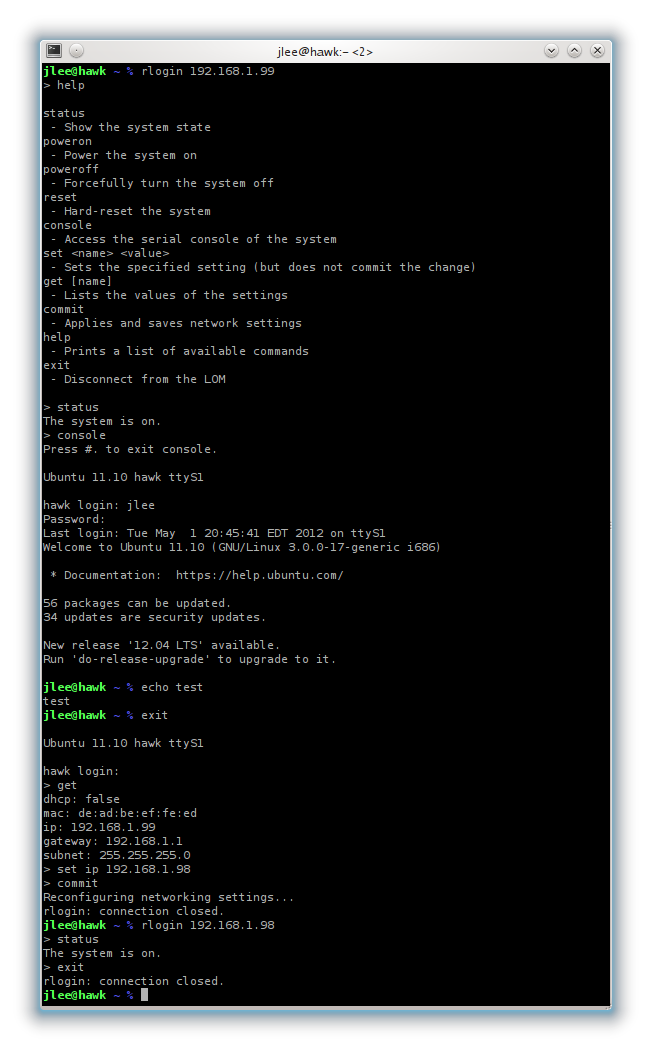
\includegraphics[height=.9\textheight]{session.png}
\end{center}

\section{Retrospective}
This project was my first introduction to SPI, and learning some of its idiosyncracies took time.  For example, with the MAX3110 command set, data is potentially returned for every read and write operation, so my driver had to be very careful about managing its internal buffers and choosing when to read and write to the UART.  If the driver received a write request, and the receive buffer is full, then I can't write anything to the UART because it may return received data which I would have no place to store.  Since the UART has a hardware FIFO buffer and the chip doesn't expose a way to check whether the FIFO buffer status is full, I chose to assume the FIFO could handle any additional received data while the user clears out the driver's receive buffer, or let the UART drop frames.  I designed my driver not to lose any data, and that helped me rule out a lot of data loss issues when it came time to integrate the serial and networking pieces of the project together.

The UART's datasheet recommends coding a driver with both a receive and transmit buffer which get filled and flushed by interrupts raised by the chip.  I tried implementing the driver that way, which worked well for received data, but often ``stuck'' for transmitted data (data wouldn't get flushed from the transmit buffer).  It seemed from my experimentation that the UART transmit buffer empty interrupt would often get raised during a receive interrupt handler, so it would get ignored.  Getting the timing right to ensure data could be both transmitted and received as a result of an interrupt seemed too hard to tackle.  Now that I know how to use an oscilloscope, I could revisit the issue with better tools to help me visualize the timing conflicts.  Ultimately, I decided that, since my program gets to choose when to transmit data, a transmit buffer (and its respective interrupt) is unnecessary.

The project also taught me how much more complicated Telnet is that I originally expected.  And, because it's basically a dead protocol that hardly anyone implements anymore, the only sources of information about the protocol are its RFC documents and old \texttt{telnetd} source code.

I also learned to not trust the compiler completely.  I ran into a bug in \texttt{avr-gcc} that caused the Arduino Ethernet library to fail on my machine.  The bug is outlined in detail at \url{http://code.google.com/p/arduino/issues/detail?id=605}.

Finally, I also learned a little bit about creating a PCB from a schematic.  Using the Eagle schematic editor, it was interesting to see the way it automatically associates packages and footprints to components on the schematic, and highlights where traces are needed.  I think I'd like to learn more about the hardware fabrication part in the future.

This project exposed me to many new concepts and I hit a lot of roadblocks along the way, but I ended up with something that works as I originally planned, and it's something that I will actually get a lot of use out of, and I am proud of that.

\end{document}
